\begin{comment}
\documentclass[10pt]{article}
\usepackage{fullpage, graphicx, url}
\setlength{\parskip}{1ex}
\setlength{\parindent}{0ex}
\title{GEN06}
\begin{document}


\begin{tabular}{ccc}
The Alternative Csound Reference Manual & & \\
Previous & &Next

\end{tabular}

%\hline 
\end{comment}
\section{GEN06}
GEN06�--� Generates a function comprised of segments of cubic polynomials. \subsection*{Description}


  This subroutine will generate a function comprised of segments of cubic polynomials, spanning specified points just three at a time. 
\subsection*{Syntax}


 \textbf{f}
 \# time size 6 a n1 b n2 c n3 d ...
\subsection*{Initialization}


 \emph{size}
 -- number of points in the table. Must be a power off or power-of-2 plus 1 (see \emph{f statement}
). 


 \emph{a, c, e, ...}
 -- local maxima or minima of successive segments, depending on the relation of these points to adjacent inflexions. May be either positive or negative. 


 \emph{b, d, f, ...}
 -- ordinate values of points of inflexion at the ends of successive curved segments. May be positive or negative. 


 \emph{n1, n2, n3 ...}
 -- number of stored values between specified points. Cannot be negative, but a zero is meaningful for specifying discontinuities. The sum \emph{n1}
 + \emph{n2}
 + ... will normally equal size for fully specified functions. (for details, see \emph{GEN05}
). 


 


\begin{tabular}{cc}
\textbf{Note}
 \\
� &

 \emph{GEN06}
 constructs a stored function from segments of cubic polynomial functions. Segments link ordinate values in groups of 3: point of inflexion, maximum/minimum, point of inflexion. The first complete segment encompasses \emph{b}
, \emph{c}
, \emph{d}
 and has length \emph{n2}
 + \emph{n3}
, the next encompasses \emph{d}
, \emph{e}
, \emph{f}
 and has length \emph{n4}
 + \emph{n5}
, etc. The first segment (\emph{a}
, \emph{b}
 with length \emph{n1}
) is partial with only one inflexion; the last segment may be partial too. Although the inflexion points \emph{b}
, \emph{d}
, \emph{f}
 ... each figure in two segments (to the left and right), the slope of the two segments remains independent at that common point (i.e. the 1st derivative will likely be discontinuous). When \emph{a}
, \emph{c}
, \emph{e}
... are alternately maximum and minimum, the inflexion joins will be relatively smooth; for successive maxima or successive minima the inflexions will be comb-like. 


\end{tabular}

\subsection*{Examples}


  Here is a simple example of the GEN06 routine. It uses the files \emph{gen06.orc}
 and \emph{gen06.sco}
. It creates a curve running 0 to 1 to -1, with a minimum, maximum and minimum at these values respectively. Inflexions are at .5 and 0 and are relatively smooth. Here is its diagram: 


 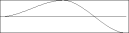
\includegraphics[scale=1]{gen06} 


 Diagram of the waveform generated by GEN06.


 \textbf{Example 1. A simple example of the GEN06 routine.}

\begin{lstlisting}
/* gen06.orc */
; Initialize the global variables.
sr = 44100
kr = 4410
ksmps = 10
nchnls = 1

; Instrument #1.
instr 1
  ; Create an index over the length of our entire note.
  kcps init 1/p3
  kndx phasor kcps

  ; Read Table #1 with our index.
  ifn = 1
  ixmode = 1
  kval table kndx, ifn, ixmode

  ; Generate a sine waveform, use our Table #1 value to 
  ; vary its frequency by 100 Hz from its base frequency.
  ibasefreq = 440
  kfreq = kval * 100
  a1 oscil 20000, ibasefreq + kfreq, 2
  out a1
endin
/* gen06.orc */
        
\end{lstlisting}
\begin{lstlisting}
/* gen06.sco */
; Table #1: a curve (using GEN06).
f 1 0 65 6 0 16 0.5 16 1 16 0 16 -1
; Table #2, a sine wave.
f 2 0 16384 10 1

; Play Instrument #1 for 2 seconds.
i 1 0 2
e
/* gen06.sco */
        
\end{lstlisting}
\subsection*{See Also}


 \emph{GEN05}
, \emph{GEN07}
, and \emph{GEN08}

%\hline 


\begin{comment}
\begin{tabular}{lcr}
Previous &Home &Next \\
GEN05 &Up &GEN07

\end{tabular}


\end{document}
\end{comment}
